\chapter{The HPS Detector}

The HPS detector is a spectrometer with a silicon vertex tracker (SVT) for momentum measurement and a electromagnetic calorimeter (ECal) for energy measurement and trigger.
The detector is installed in the middle dipole of a three-magnet chicane, with the field extending from the target foil to the end of the tracker.

The detector design is determined by physics needs.
To capture low-mass $A'$, the detector must have acceptance at small angles from the beam.
To get the best possible vertex resolution, the detector must operate as close to the target as possible.
Because multiple scattering dominates tracking resolution at HPS energies, the material in the tracking volume must be kept as low as possible.

Elastic scatters in the target send large numbers of electrons into the detector acceptance, so it needs to tolerate high rates and have a selective trigger.
Beam-gas interactions would create large detector backgrounds and fake $A'$ decays downstream of the target, so the beam must travel in vacuum all the way through HPS.
Bremsstrahlung energy losses in the target cause beam electrons to bend in the dipole field, forming a ``sheet of flame.'' To avoid this, no detector material is placed in the beam plane.

All parts of the HPS detector have the same minimum angle, or ``dead zone,'' at 15 milliradians.
This is set by the maximum rate tolerable in the first layer of the SVT: the occupancy within a resolution-limited hit time window must be less than 1\% for clean track reconstruction, and radiation damage must be kept low enough that the SVT remains fully functional after six months of operation.

\begin{figure}[ht]
    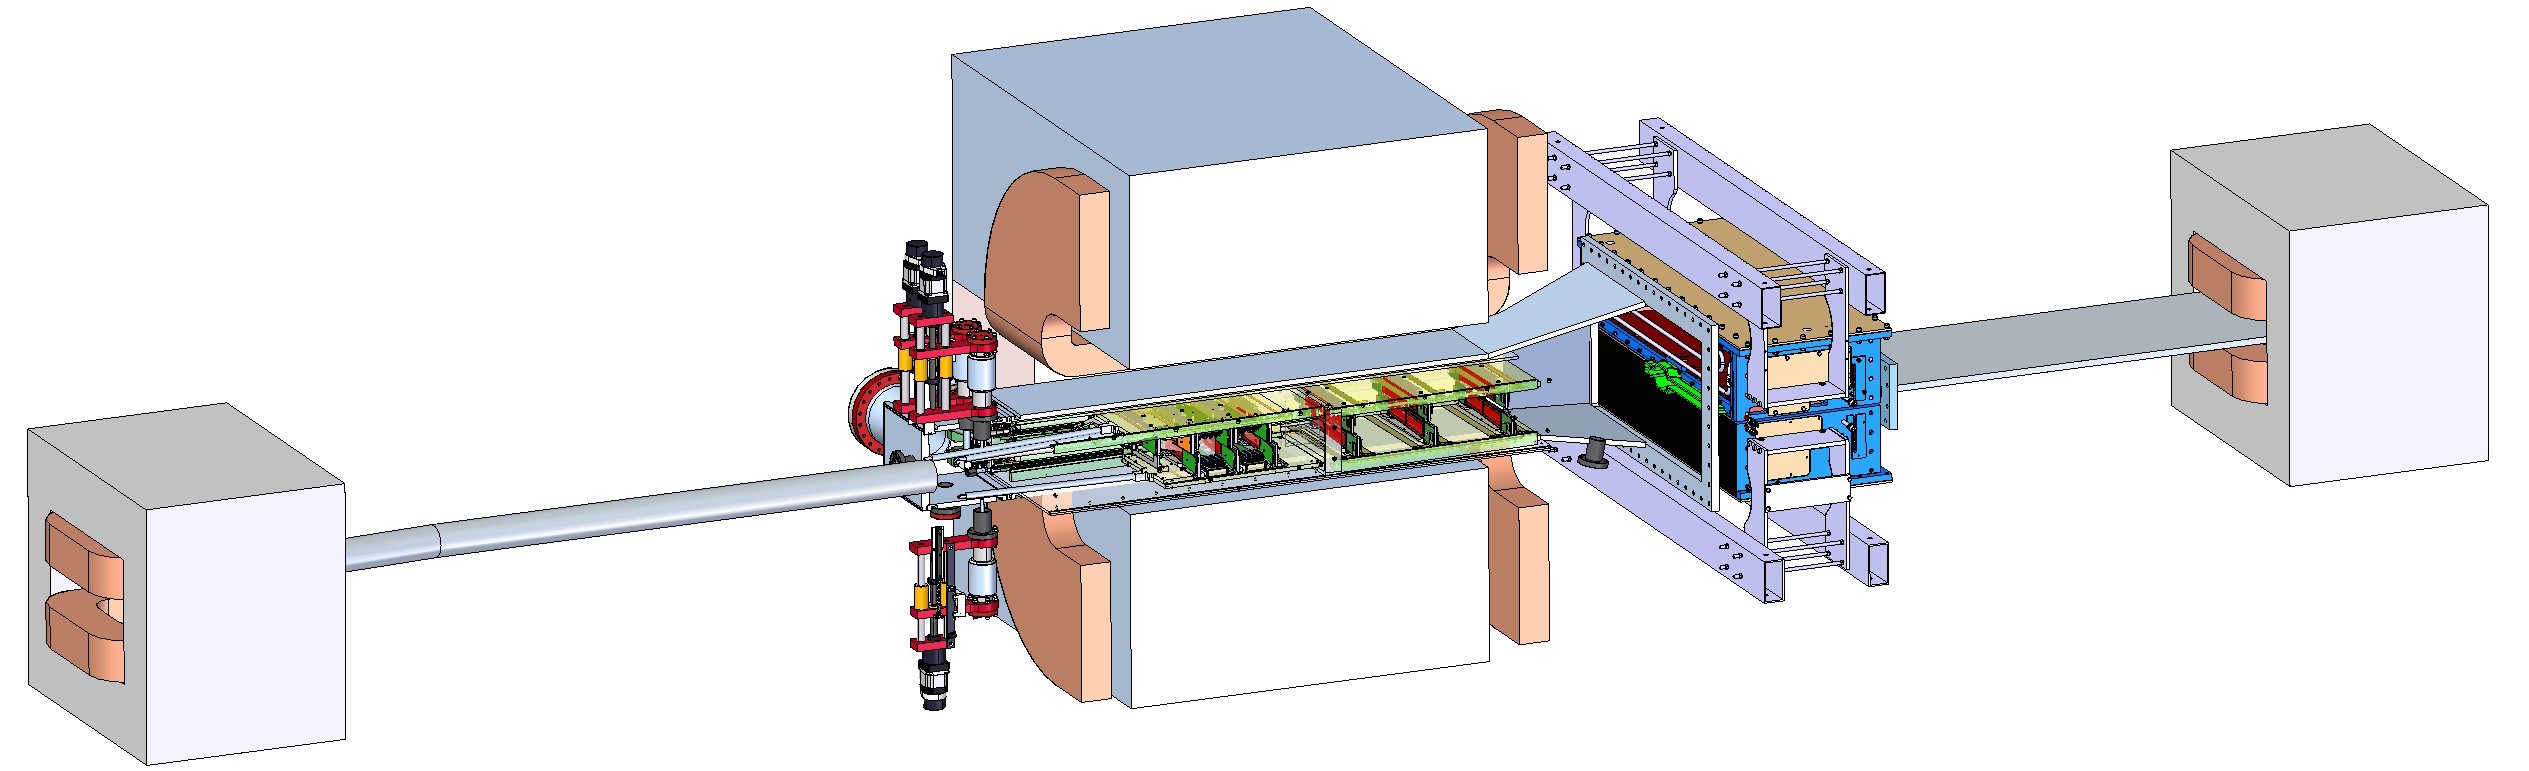
\includegraphics[width=\textwidth]{detector/figs/HPS-pic}
    \caption{View of the HPS setup.}
    \label{fig:hps-pic}
\end{figure}

\begin{figure}[ht]
    \begin{center}
        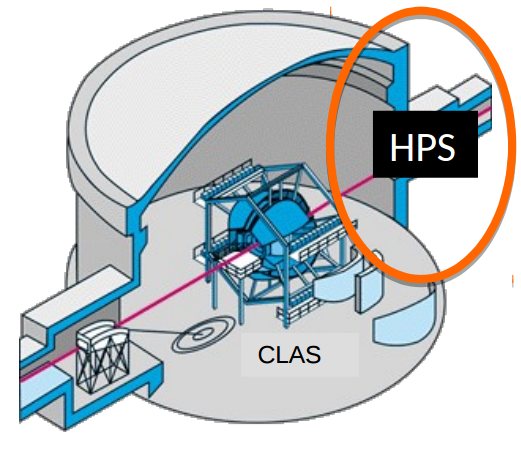
\includegraphics[width=0.5\textwidth]{detector/figs/hallb}
    \end{center}
    \caption{Location of the HPS setup in Hall B.}
    \label{fig:hallb}
\end{figure}

\section{Beamline}

HPS uses the CEBAF (Continuous Electron Beam Accelerator Facility) accelerator at Jefferson Lab (Figure \ref{fig:cebaf}).
CEBAF is a recirculating linac, where the electron beam can take multiple passes through the same set of accelerating cavities.
%CEBAF has a continuous duty cycle because it uses superconducting accelerating cavities, which can be operated continuously without 
The superconducting RF cavities used at CEBAF allow a continuous duty cycle, where beam bunches pass through the accelerator at 1500 MHz without interruption.
A system of RF separators delivers beam to each of four experimental halls at 250 or 500 MHz, and allows each hall to select its own beam energy.
HPS is installed in Hall B, in the downstream alcove of the hall (see Figure \ref{fig:hallb}).

The injector energy is 100 MeV and one pass through the linacs adds 2.2 GeV to the beam energy, so in normal operation, the available beam energies at Hall B are 100 MeV + $n*2.2$ GeV where $n$ is 1 through 5.
During the 2015 engineering run, a mechanical problem disabled one of the two CEBAF helium liquifiers.
With half the cooling power, the superconducting cavities could only be run at half the nominal gradient.
HPS took the opportunity to run at 1.056 GeV, an energy that is not normally available.

HPS relies on the continuous beam structure at CEBAF to reduce pileup.
A beam bunch arrives at HPS every 2 ns, which is comparable to the time resolution of the detectors.
This means that beam backgrounds are spread in time as uniformly as possible.
A larger bunch spacing or lower duty cycle would increase the amount of beam background that overlaps an event of interest.


\begin{figure}[ht]
    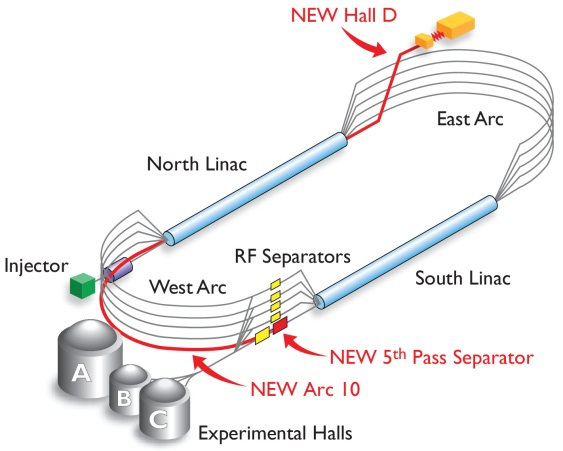
\includegraphics[width=0.6\textwidth]{detector/figs/cebaf}
    \caption{Schematic of the CEBAF accelerator, highlighting components added for the 12 GeV upgrade.}
    \label{fig:cebaf}
\end{figure}

\subsection{Target}

target

beam quality

beam diagnostics

protection

\section{Silicon Vertex Tracker}
The silicon vertex tracker (SVT) measures track momentum and vertex position.

HPS uses silicon microstrips because they provide good time resolution, low mass, and high rate.
Because a microstrip sensor can only make a 1-D measurement (it identifies the strip that was hit, but not the hit position along the strip), each measurement station (called a ``layer'') uses two sensors at an angle relative to each other.
For HPS this stereo angle is kept small, so all sensors have their strips pointing roughly in the bend direction.
A small stereo angle is a compromise: it sacrifices measurement resolution in the strip direction, but it is less likely that two particles will create ``ghost hits'' when the strips they hit intersect.
The stereo angle is not uniform throughout the SVT (it is 100 milliradians in the upstream half, 50 milliradians in the downstream half), which prevents ghost hits from creating ghost tracks.

The SVT is made up of six layers at different distances from the target: this number allows for 5-hit tracking even if a particle misses one layer.
Layer 1 is at 10 cm from the target; this is the closest we can safely operate while allowing 500 $\mu$m distance from the beam to the edge of the sensors, which have a 1 mm border of inactive silicon.
Layer 6 is at 90 cm from the target, just at the end of the uniform field region of the analyzing magnet; maximizing the length of the tracker maximizes the momentum resolution.
Layers 1--3 use single sensors; layers 4--6, where tracks have bent out to the sides, use two sensors joined end to end.

Because the SVT operates in a high magnetic field and in vacuum, materials must be compatible.
All materials are checked for vacuum compatibility by pumping test samples to high vacuum in a test chamber.
Only nonmagnetic materials are used; inductors used on the frontend boards are air-core (instead of ferrite, which would saturate).

\subsection{Sensors and Readout}
HPS uses silicon microstrip sensors that were originally produced for the run IIb upgrade of the D{\O} detector at Fermilab.
This upgrade would have replaced the entire SMT (silicon microstrip tracker).
The full SMT upgrade was cancelled in favor of an insertable Layer 0, but not before sensors had already been procured.
The sensors used for HPS are those that would have been used for layers 2--5 of the new D{\O} tracker.

The HPS sensors are single-sided p+n with AC-coupled readout: the bulk is lightly doped n-type silicon with $<$100$>$ crystal orientation, and the strip implants are strongly p-type doped.
The strips are biased through polysilicon resistors at the ends of the strips, and capacitively coupled to aluminum readout strips that run on top of the strips.
Only every other strip is read out; the ``readout'' strips capacitively couple to the intermediate ``sense'' strips.

Radiation damage limits the useful lifetime of silicon sensors.
Incident particles can displace silicon atoms from their places in the crystal lattice, which effectively converts the n-type bulk of the sensor to p-type (type inversion).
This increases the depletion voltage, so the sensor bias must be increased to keep the same charge collection efficiency; the sensor lifetime is therefore limited by the breakdown voltage of the sensor.
The defects also increase the leakage current, which leads to increased sensor heating.
The HPS sensors are specified to have a breakdown voltage of greater than 350 V, and a further selection was made to only use sensors with a breakdown voltage in excess of 1000 V.

\begin{table}[h]
    \begin{center}
        \begin{tabular}{lc}   
            \hline \hline
            Thickness & 320 $\mu$m \\
            Overall area (L$\times$W) & 100 $\times$ 40.34 mm\\
            Active area (L$\times$W) & 98.33 $\times$ 38.34 mm\\
            Strip pitch (count) & 30 $\mu$m (1277)\\
            Readout pitch (count) & 60 $\mu$m (639)\\
            Depletion voltage & 110-130 V (typical)\\
            Breakdown voltage & $>$1000 V\\
            \hline \hline
        \end{tabular}
        \caption{Specifications of the SVT sensors.
        Breakdown voltage specification is value accepted for use in HPS; procurement specification was looser.}
        \label{tab:sensor_spec} 
    \end{center}
\end{table}

\begin{table}[h]
    \begin{center}
        \begin{tabular}{lcccccc}   
            \hline \hline 
            Layer number & 1 & 2 & 3 & 4 & 5 & 6 \\      
            \hline
            nominal $z$, from target (cm)  & 10 & 20 & 30 & 50 & 70  & 90 \\ 
            Stereo Angle (mrad)  & 100 & 100 & 100 & 50 & 50 & 50 \\ 
            Bend-plane resolution ($\mu m$)  & $\approx$60 & $\approx$60 & $\approx$60 & $\approx$120 & $\approx$120 & $\approx$120 \\ 
            Non-bend resolution ($\mu m$)  & $\approx$6 & $\approx$6 & $\approx$6 & $\approx$6 & $\approx$6  & $\approx$6 \\ 
            Number of sensors  & 4 & 4 & 4 & 8 & 8 & 8 \\ 
            Nominal dead zone in $y$ (mm)  & $\pm1.5$  & $\pm3.0$  & $\pm4.5$  & $\pm7.5$  & $\pm10.5$ & $\pm13.5$  \\ 
            Module power consumption (W) & 6.9 & 6.9 & 6.9 & 13.8 & 13.8 & 13.8 \\
            \hline \hline
        \end{tabular}
        \caption{Layout of the HPS SVT.  The angle of stereo sensors is relative to the bend plane.}
        \label{tab:svt_layout} 
    \end{center}
\end{table}

The sensors are read out by the APV25 readout chip \cite{french_design_2001}.
This chip was developed for silicon microstrip readout in the CMS tracker.
Because the APV25 can read out multiple consecutive samples of its shaper waveform, it can be used for pileup rejection and high-precision hit time reconstruction.
This is an essential feature for HPS and other experiments (notably the Belle II SVD \cite{liu_belle_2012}) with CW beam and high pileup.

Each APV25 chip has 128 input channels.
One channel consists of a charge-sensitive preamp with an optional inverter, CR-RC shaper, and 192-cell analog pipeline.
We run the chip with a 24 ns clock: the design clock period is 25 ns to match the LHC bunch crossing period, but 24 ns is an even multiple of the standard JLab clock.
On each clock, each channel samples its shaper output and stores it in a cell of its pipeline.
On a trigger, each channel reads out the appropriate pipeline cell, and the chip multiplexes the 128 signals onto a single differential current output.

\begin{figure}[ht]
    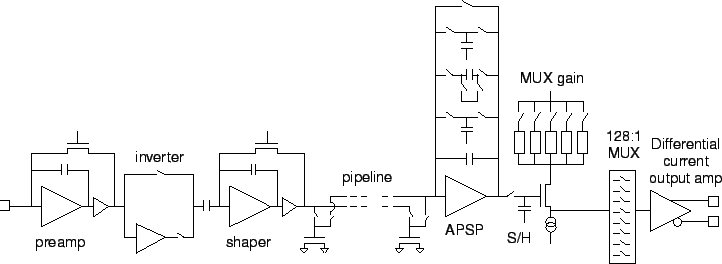
\includegraphics[width=\textwidth]{detector/figs/apv25}
    \caption{Schematic of the APV25. The APSP (analog pulse shape processor) is disabled in the ``multi-peak'' readout mode used by HPS.}
    \label{fig:apv25}
\end{figure}


\subsection{Mechanical Support}
The base unit of the SVT is a ``half-module'' comprising a low-mass support structure, sensors, and hybrid readout circuit boards.
Half-modules are the only unit of the SVT that cannot be disassembled and reworked.
Two types of half-modules are used: layers 1--3 use single-ended half-modules with one sensor and hybrid each, and layers 4--6 use double-ended half-modules with two sensors and hybrids each.
A single half-module provides a single measurement (axial or stereo) for one half (top or bottom) of a layer.

The hybrid circuit board carries the APV25 readout chips, and connects the sensor to the rest of the DAQ.
The input channels of the APV25 chips are wirebonded directly to the sensor; the APV25 power, output channels, and control lines are wirebonded to the hybrid.
The hybrid also carries filter capacitors for the sensor bias, and temperature sensors to monitor the sensor temperature.

The carbon fiber support structure provides structural support for the silicon, and acts as a ground plane for the half-module.
A layer of Kapton insulation isolates the carbon fiber from the back surface of the sensor, which is held at high voltage.
The carbon fiber and Kapton are thinner than the silicon and contribute negligibly to the material seen by particles; cutouts further reduce any effect.
The sensors and hybrids are glued to the support structure with epoxy.

Two half-modules are paired back-to-back to form a ``module.''
The axial half-module is oriented with its strips pointing in the bend direction; the stereo half-module is rotated so it dips into the beam plane on the positron side (where beam backgrounds are less intense).
The modules are assembled using pairing fixtures, which are machined to set the edges of the sensors at precisely the correct height and angle.

The aluminum module support holds the half-modules at both ends.
Heat generated by the hybrids is pulled out through the module support, which is in close thermal contact with the APV25 chips and the sensors through parallel paths so that the sensors can be kept colder than the APV25 chips.
The module support and the half-modules contract at different rates when the SVT is cooled to its operating temperature, so the module support must apply constant tension to keep the half-modules flat.
This is done with a spring pivot on one side of the module support.

Three modules are mounted on a common aluminum support structure to form a ``U-channel.''
The sidewalls add to the rigidity of the U-channel and shield the sensors from thermal radiation.
The module mounting surfaces are recessed by the correct amounts to put the layers at the correct distances from the beam.
The SVT is divided into four U-channels: top and bottom L1--3, top and bottom L4--6.

Each U-channel is supported at three points using kinematic mounts, which guarantee repeatable positioning when the U-channels are installed.
The L4--6 U-channels rest on three kinematic mounts.
The L1--3 U-channels rest on two kinematic mounts, which serve as a hinge at the downstream end of the U-channels, and are supported on the upstream end by motion levers which tilt the U-channels up and down.
In addition to modules, the L1--3 U-channels carry scan wires so that the beam position can be measured relative to the silicon.

\subsection{Power and Data Acquisition}
The power and data paths for the SVT are constrained.
All signals must pass through a pair of 8-inch vacuum flanges at the upstream side of the analyzing magnet, so the number of signals has to be reduced.
The closest available rack for the SVT power supplies and DAQ is 20 meters from the alcove where HPS is installed, so the analog APV25 output signals have to be converted to digital optical signals.
Therefore HPS digitizes the signals and regulates the low-voltage power supplies inside the vacuum chamber, on frontend boards (FEBs) that are mounted on a cooling plate next to layers 1--3.

Each FEB can service four hybrids: a pair of L1--3 modules or a single L4--6 module.
A single bundle of impedance-controlled twisted pair magnet wire connects each FEB to its set of hybrids, carrying low-voltage power, high-voltage sensor bias, analog APV25 output signals, and digital control and trigger signals.

Each FEB digitizes the output signals from 20 APV25 chips.
Each differential current signal is converted to a voltage by a preamp and digitized by a 14-bit ADC.
Each FEB carries a single Xilinx Artix-7 FPGA, which packs the ADC data to be streamed off the FEB.
The FPGA also monitors the hybrid state and configuration.
All data and control signals are on a single high-speed data link, carried by a standard mini-SAS cable.

The FEBs also distribute low-voltage power to the hybrids.
A single voltage supplied to the FEB is split into four independent voltages (one per hybrid) using a combination of switching and linear voltage regulators.
This improves noise performance and reduces the number of voltages that must be passed into the vacuum chamber.
High-voltage sensor bias is also routed through the FEBs, but is passed through directly.

Two sets of cables connect the FEBs to the vacuum chamber flanges: mini-SAS cables carrying digital signals, and twisted pair cables carrying low-voltage power and high-voltage bias.
In both cases, the number of connections is too high for conventional vacuum feedthroughs.
Instead, HPS uses ``flange boards.''
Each board has a vacuum side and an air side, to which connections are made using solder or standard connectors.
The middle section of the board carries signal traces but is kept smooth; the board is then passed through a machined gap in the vacuum flange, and epoxy is poured to fill the space around the board: see Figure \ref{fig:flangeboard_test}.
The flange on beam-right carries two flange boards: one for low voltage and one for high voltage.
The flange on beam-left carries four signal flange boards (one of which is shown in Figure \ref{fig:flangeboard}), which use fiber transceivers on the air side to convert the electrical signals to optical signals.

The low and high voltages for the SVT are supplied by Wiener MPOD power supplies.
The low-voltage supplies use sense lines to regulate the voltage actually supplied to the FEBs, and compensate for voltage drop in the cables.

The core of the SVT DAQ is the RCE platform.
This is a general-purpose DAQ system developed at SLAC.
The system is built on the ATCA (Advanced Telecommunications Computing Architecture) industry standard and is housed in a standard ATCA crate.

The data processing, trigger handling, and event building is done on a COB (Cluster On Board) blade, which carries a set of daughterboards: four DPMs (Data Processing Modules) and one DTM (Data Transport Module).
All of these are generic hardware that can be used for any experiment using the RCE platform.
The only HPS-specific hardware is the (RTM) Rear Transition Module, which interfaces the COB to the fiber bundles connected to the signal flange boards.
The SVT DAQ uses two fully loaded COBs and two RTMs.
Each DPM contains two data processing nodes, each of which runs a Xilinx Zynq system-on-a-chip which integrates an ARM processor (running the Linux operating system) and an FPGA.
The nodes can therefore process and reduce data on the FPGA at high speed, and perform high-level functions on the processor.
The DTM contains a single node, which handles timing and trigger distribution.
An implementation of the JLab TI (Trigger Interface) module is integrated in the DTM firmware for HPS.

\subsection{Services}


\begin{figure}[ht]
    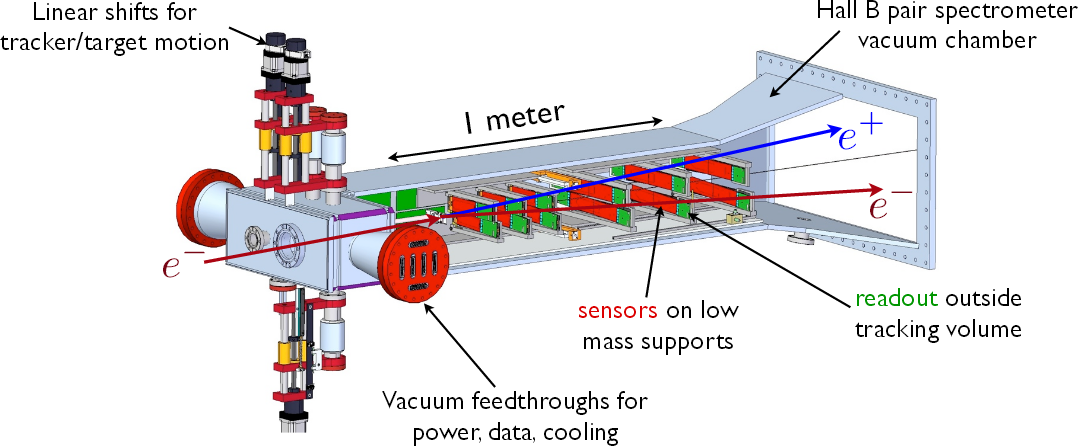
\includegraphics[width=\textwidth]{detector/figs/svt_cutaway}
    \caption{Schematic of the SVT and its support systems.}
    \label{fig:svt-schematic}
\end{figure}

\begin{figure}[ht]
    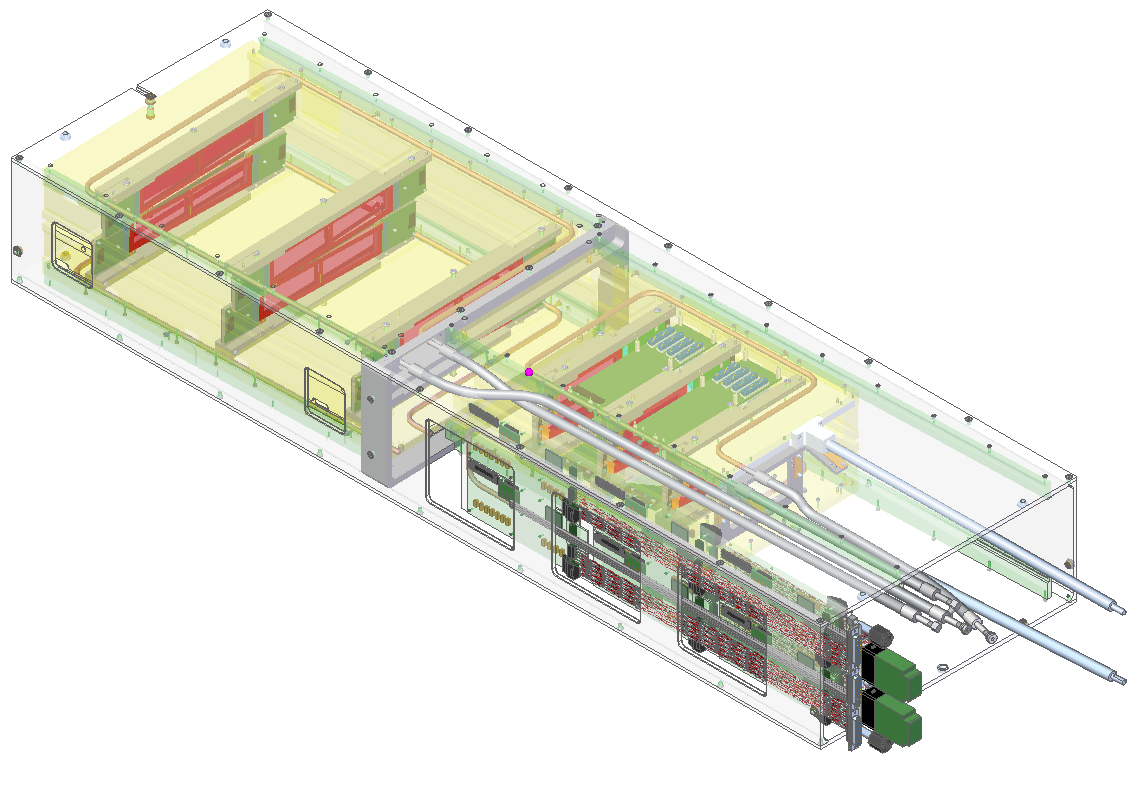
\includegraphics[width=\textwidth]{detector/figs/svt_drawing}
    \caption{Rendering of the SVT as built, showing cooling lines and motion levers.}
    \label{fig:svt-drawing}
\end{figure}

\begin{figure}[ht]
    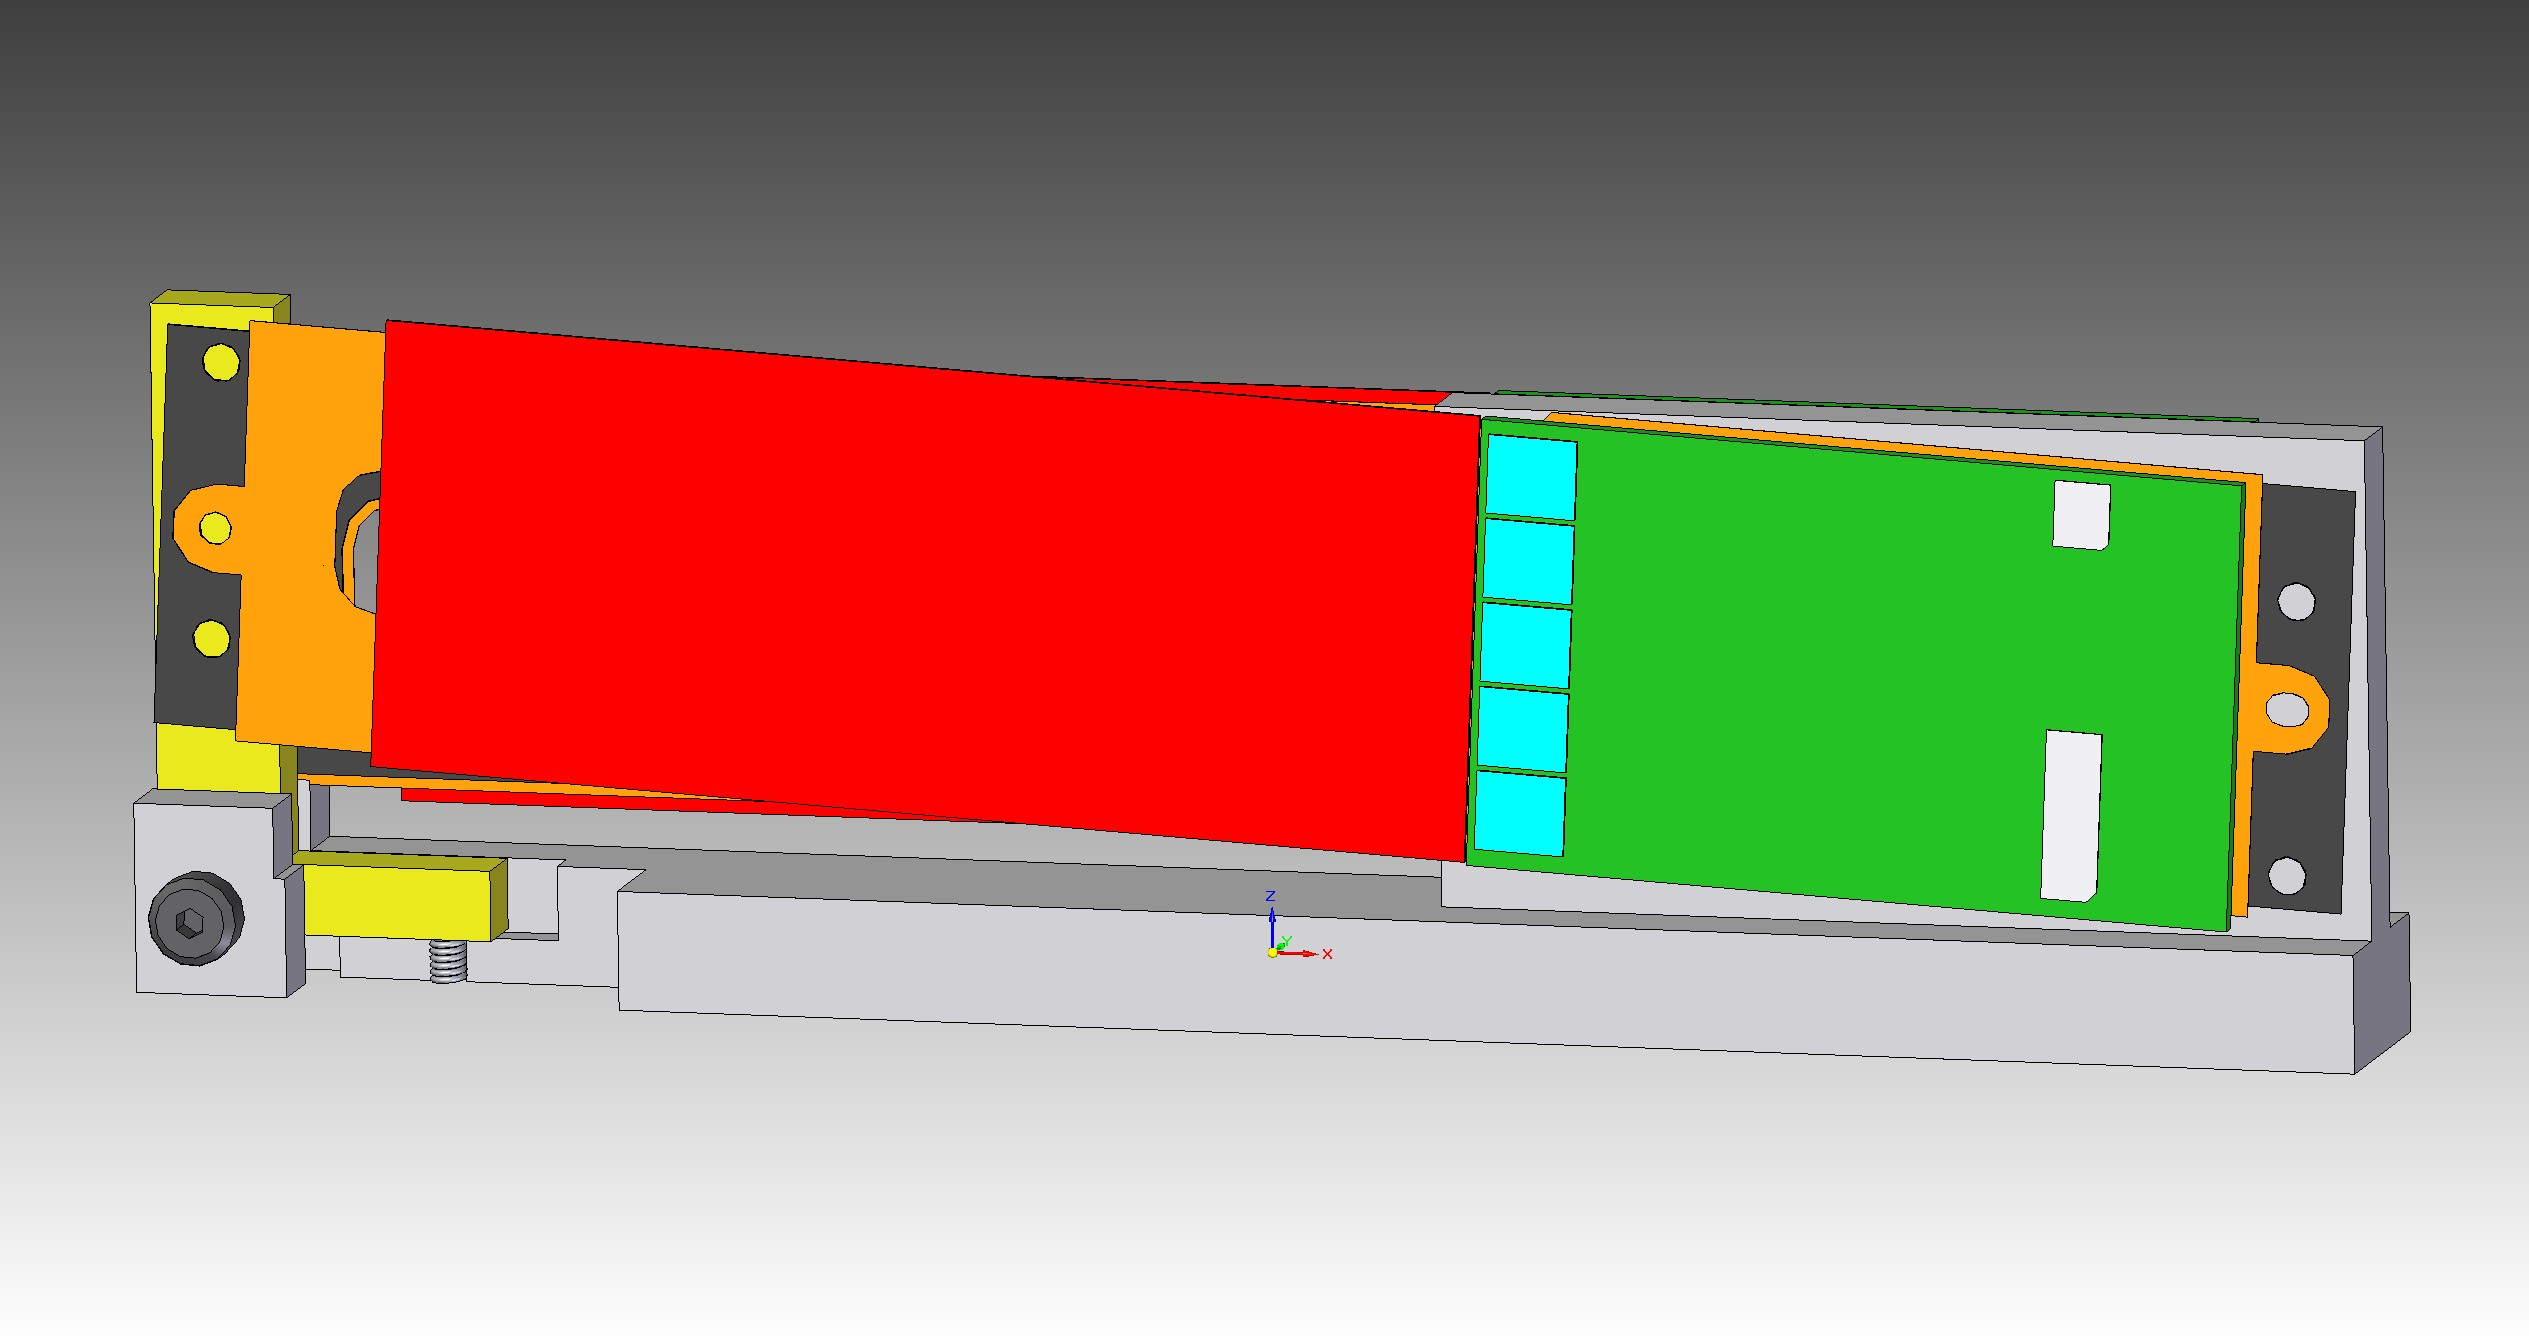
\includegraphics[width=0.5\textwidth]{detector/figs/svt_l123_drawing}
    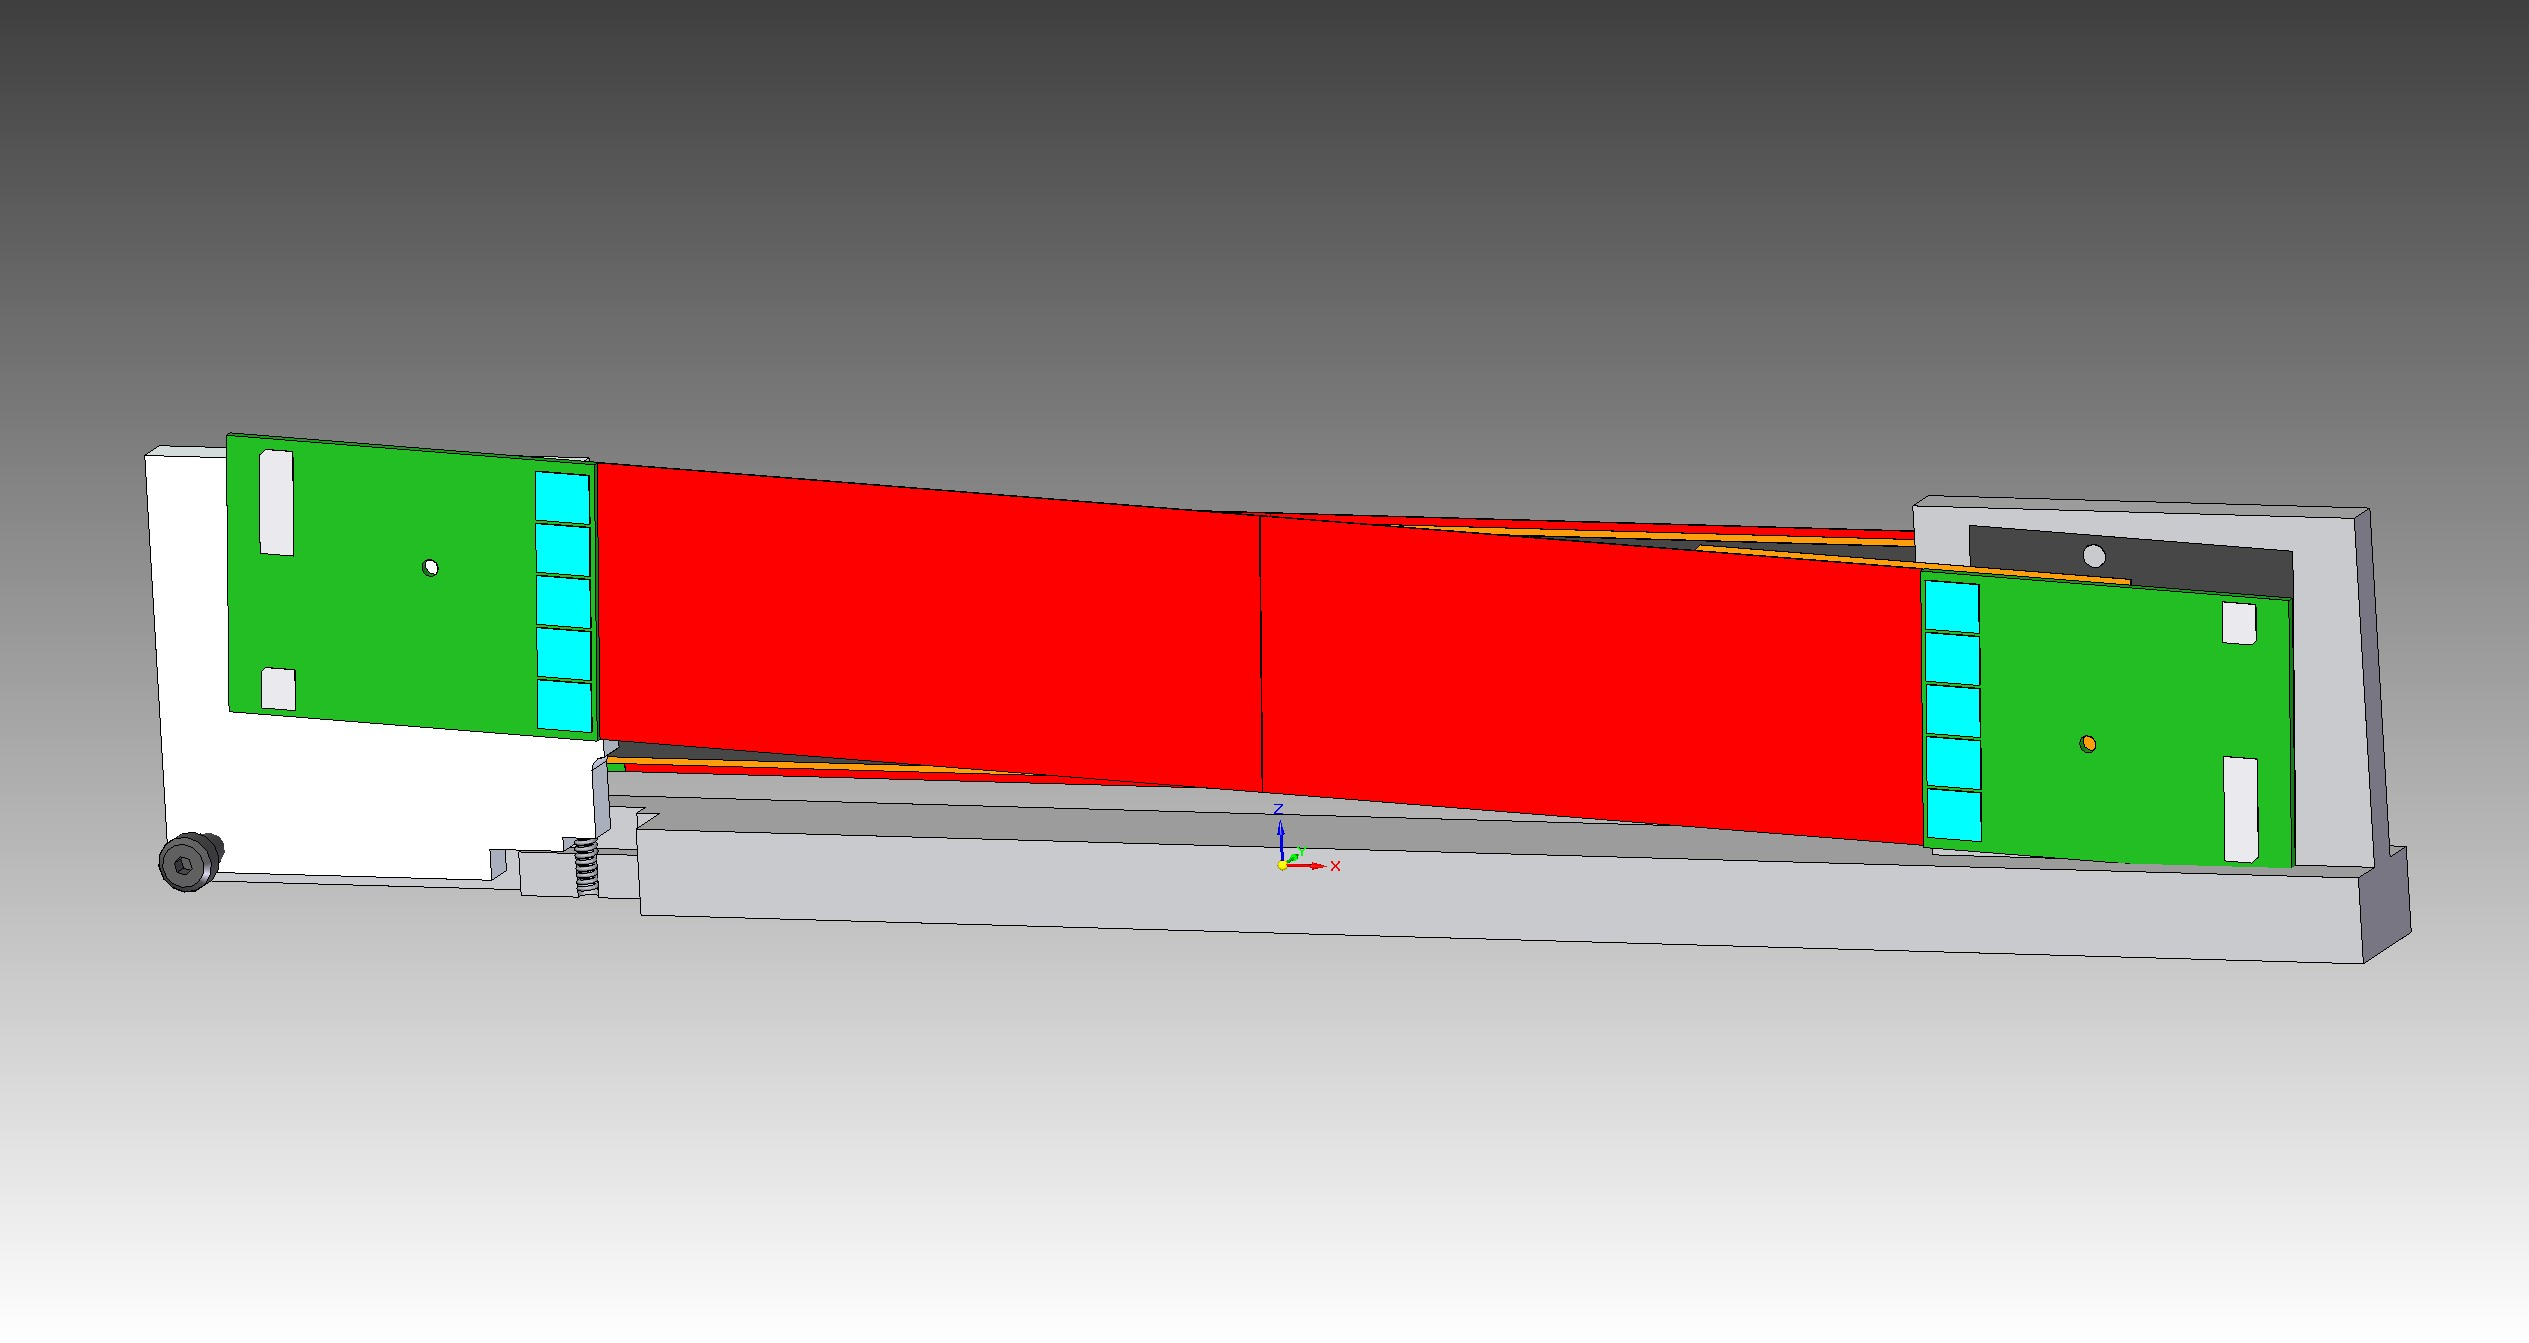
\includegraphics[width=0.5\textwidth]{detector/figs/svt_l456_drawing}
    \caption{Renderings of the L1--3 (left) and L4--6 (right) module designs, with cutaways to show the spring pivots that hold the silicon under constant tension.}
    \label{fig:svt-module-drawing}
\end{figure}

\begin{figure}[ht]
    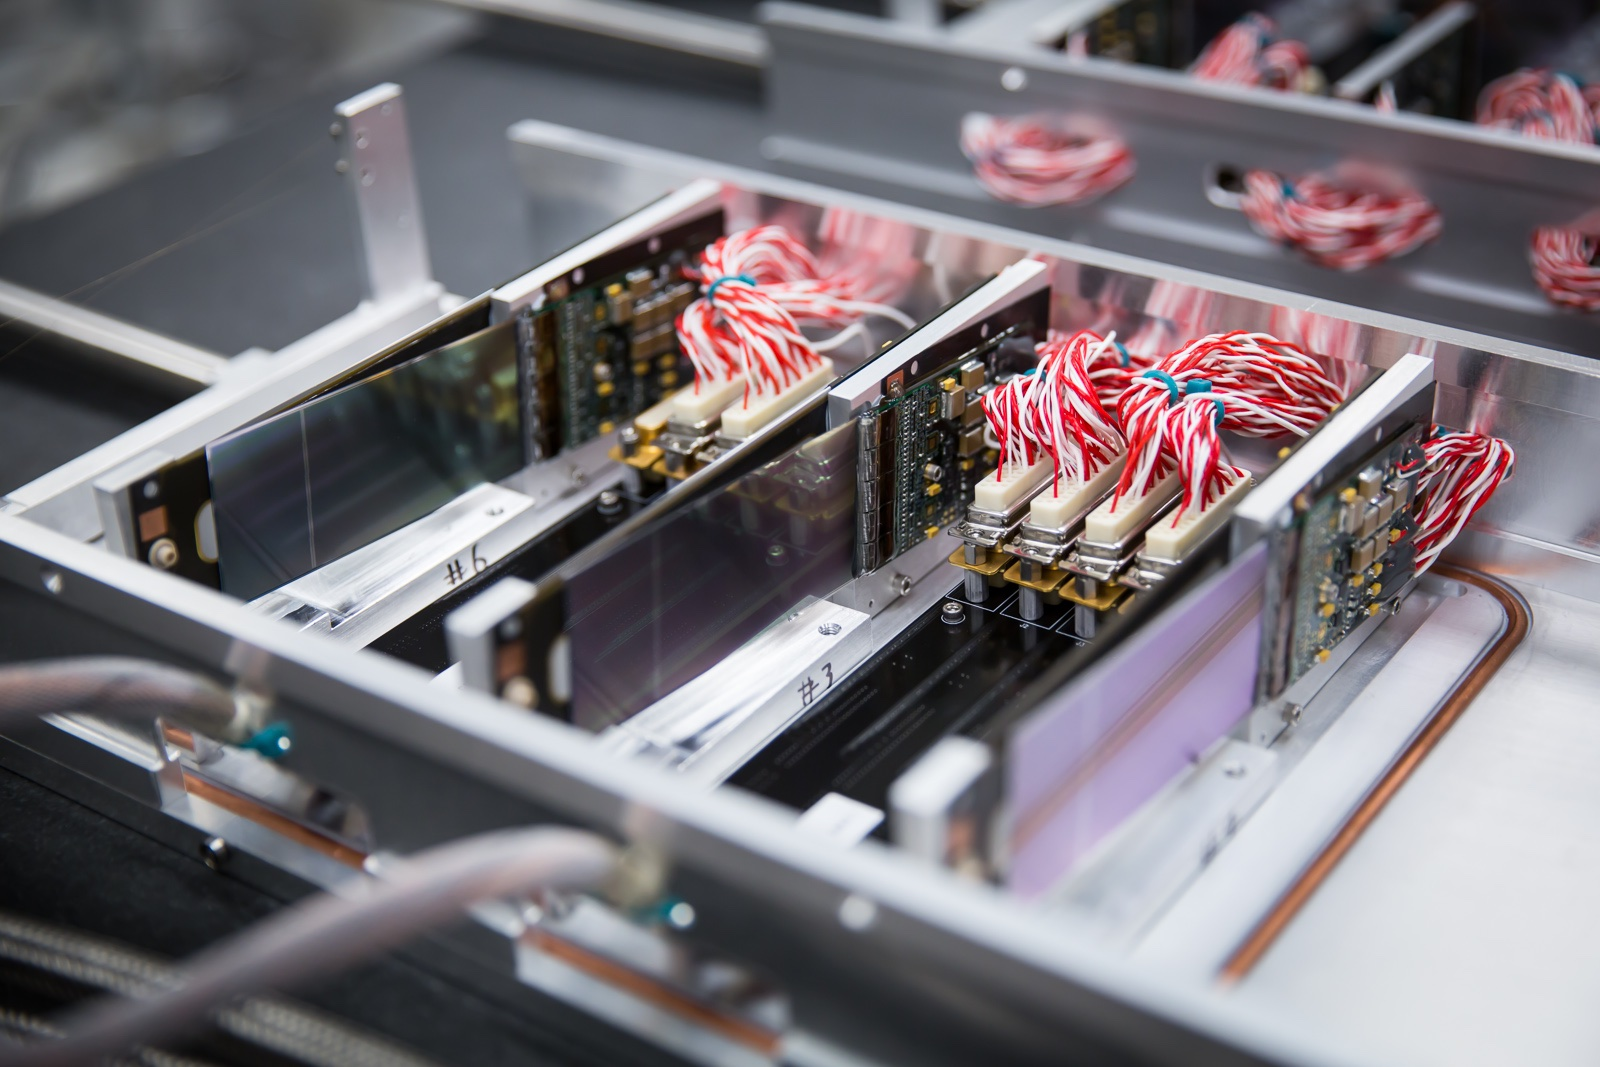
\includegraphics[width=\textwidth]{detector/figs/l123}
    \caption{One of two U-channels for L1--3, fully assembled.}
    \label{fig:l123}
\end{figure}

\begin{figure}[ht]
    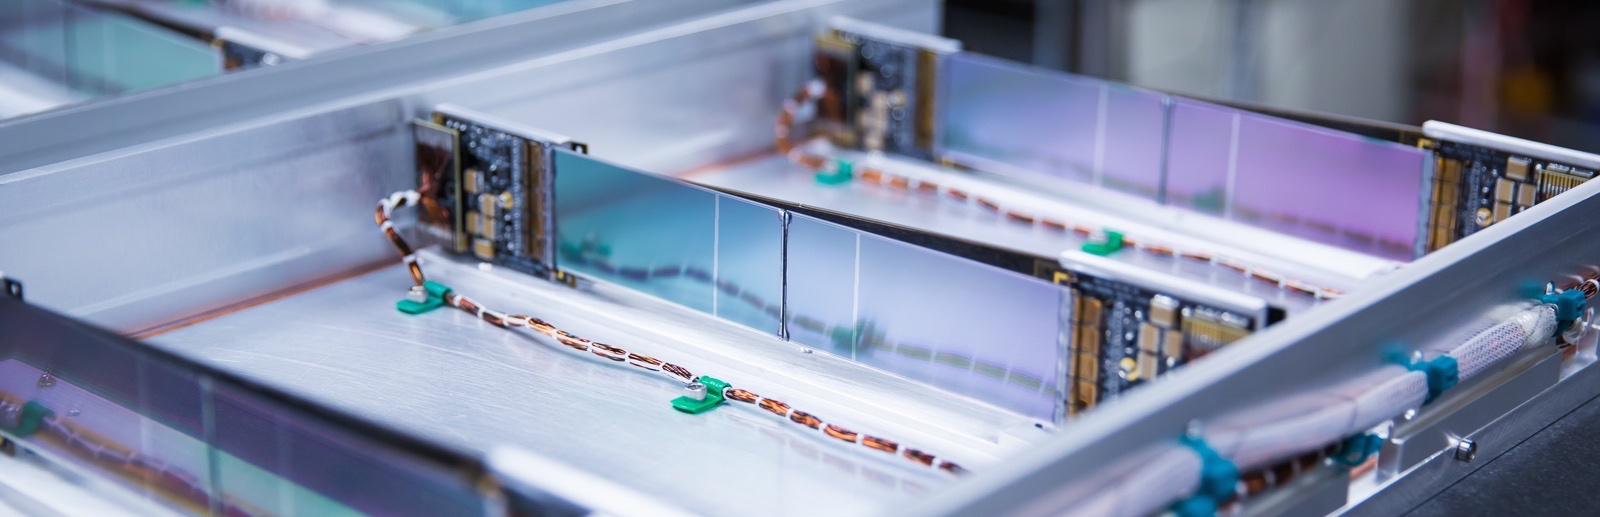
\includegraphics[width=\textwidth]{detector/figs/l456}
    \caption{One of two U-channels for L4--6, fully assembled.}
    \label{fig:l456}
\end{figure}

\begin{figure}[ht]
    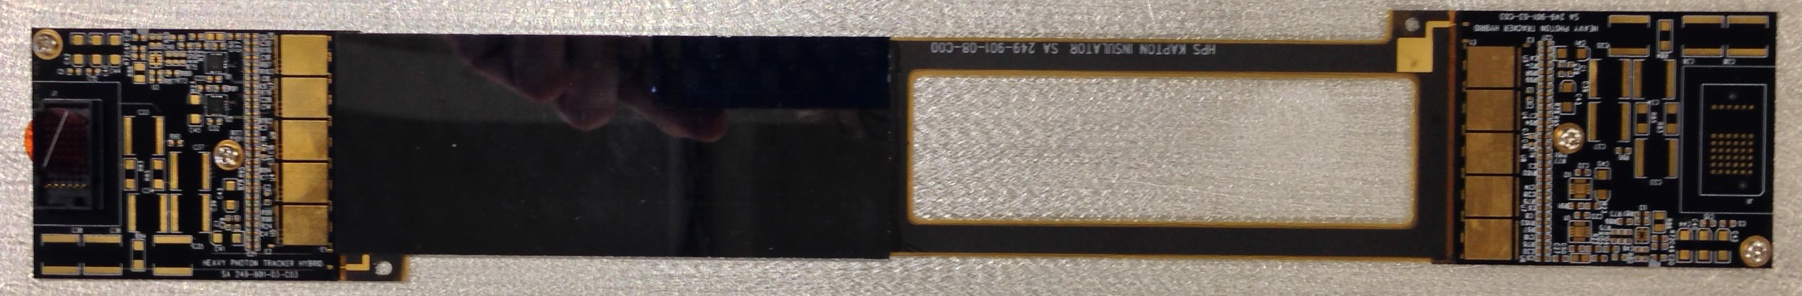
\includegraphics[width=\textwidth]{detector/figs/l456_hm}
    \caption{One half-module for L4--6. The two hybrids (without readout chips, which would be mounted on the gold pads) are at the left and right ends. One sensor is in place, on the left. The carbon fiber support and Kapton passivation layer are visible on the right.}
    \label{fig:l456_hm}
\end{figure}

\begin{figure}[ht]
    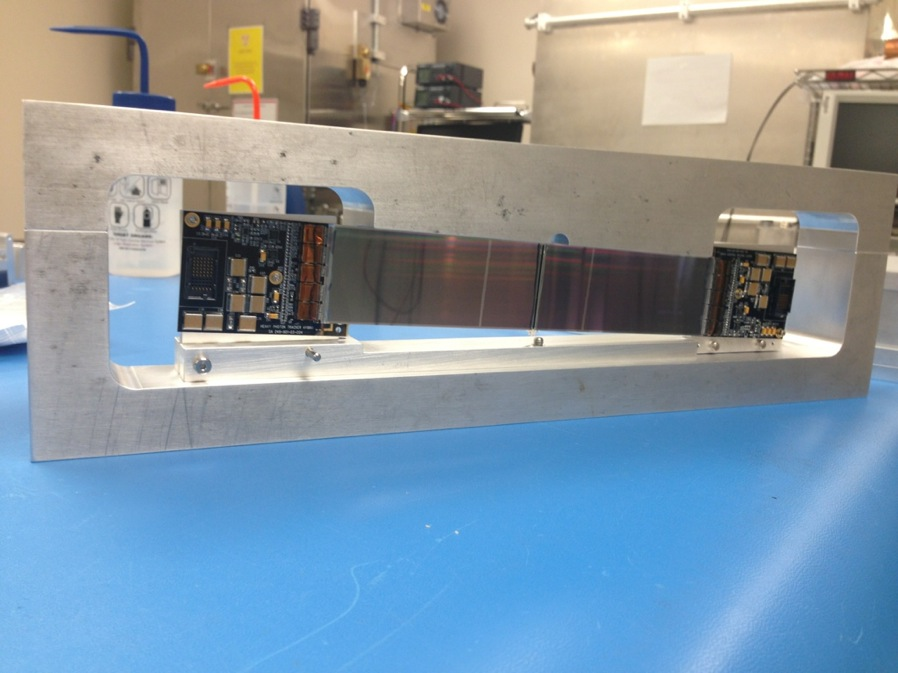
\includegraphics[width=\textwidth]{detector/figs/pairing_l456}
    \caption{The L4--6 pairing fixture, with one half-module in place.}
    \label{fig:l456_pairing}
\end{figure}

\begin{figure}[ht]
    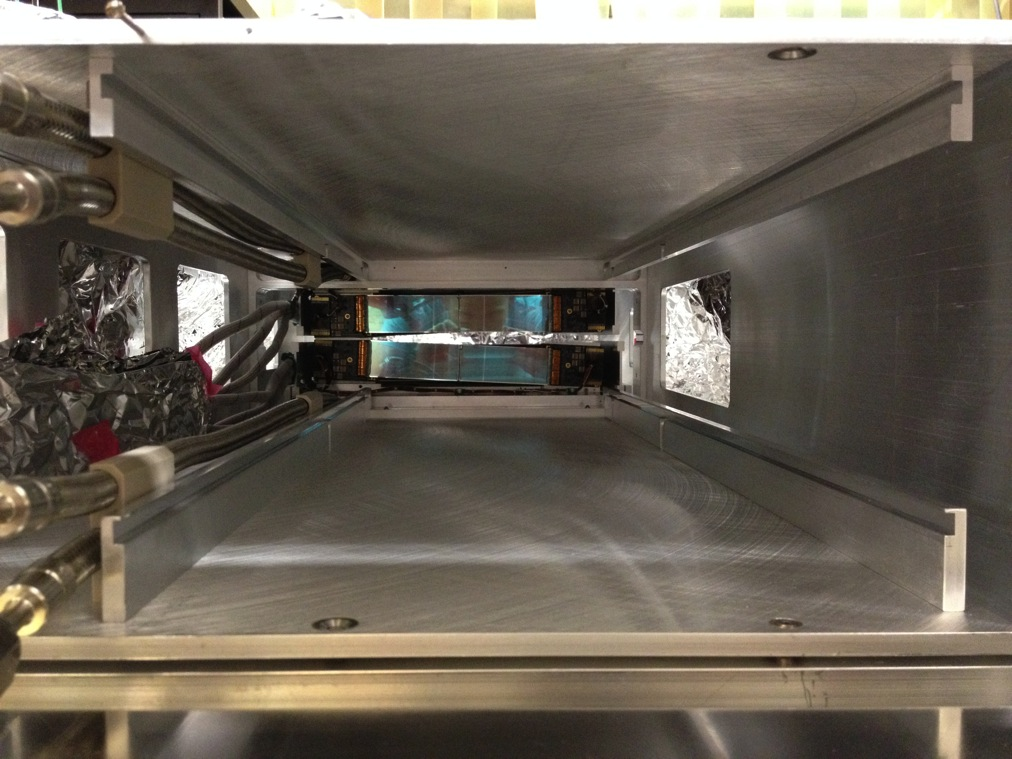
\includegraphics[angle=90,width=\textwidth]{detector/figs/drawers}
    \caption{Inside the SVT box, looking downstream.
    The L4--6 U-channels are installed.
The rails for the L1--3 U-channels can be seen at the top and bottom. When the U-channels are installed, bearings on the U-channels roll along the horizontal slots until they drop down into the vertical slots, guiding the U-channel onto its kinematic mounts.}
    \label{fig:drawers}
\end{figure}

\begin{figure}[ht]
    %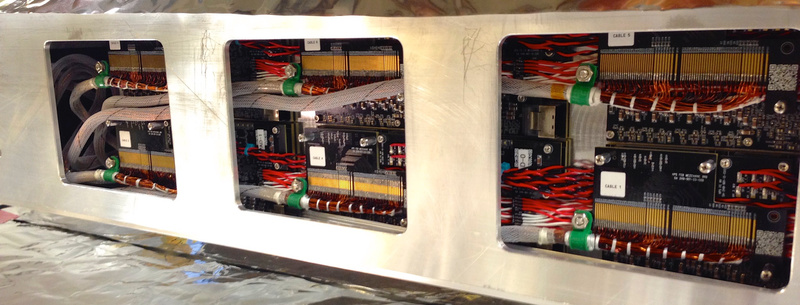
\includegraphics[width=\textwidth]{detector/figs/svt_febs}
    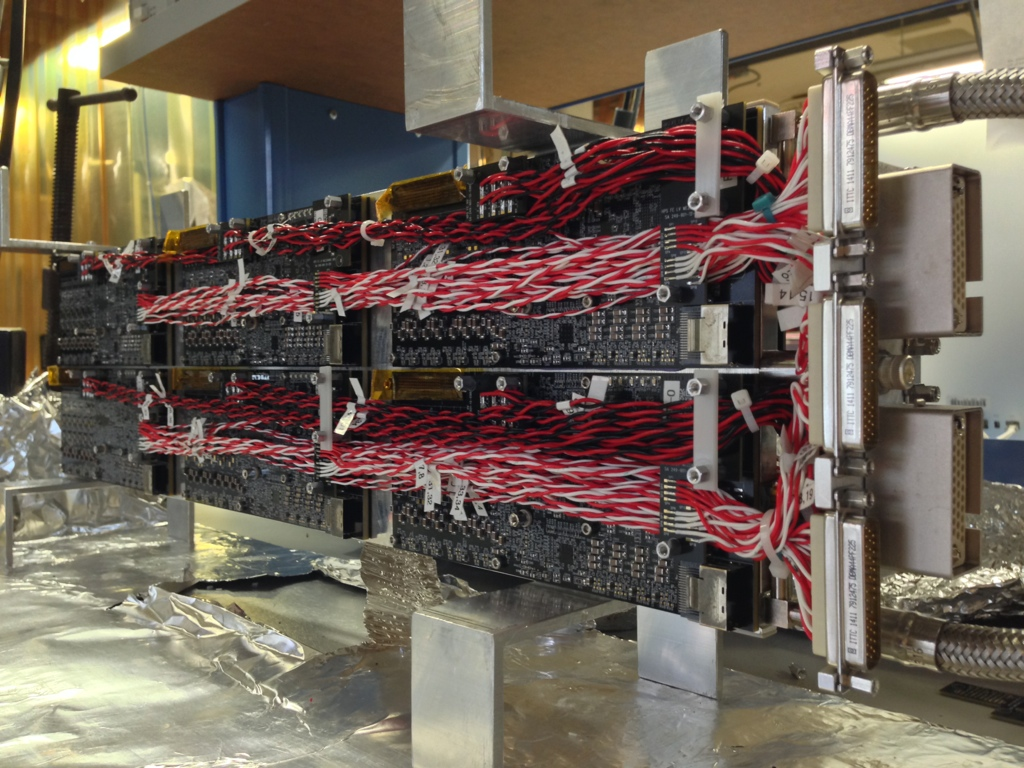
\includegraphics[width=\textwidth]{detector/figs/febplate}
    \caption{The SVT FEBs (frontend boards), mounted on their cooling plate. The red-and-white cables distribute low-voltage power to the FEBs; the red-and-black cables distribute high-voltage bias to the FEBs. The connectors for hybrid power, bias and data are covered with yellow Kapton tape. The mini-SAS connectors for high-speed data cables are at the bottom right of each FEB.}
    \label{fig:febplate}
\end{figure}

\begin{figure}[ht]
    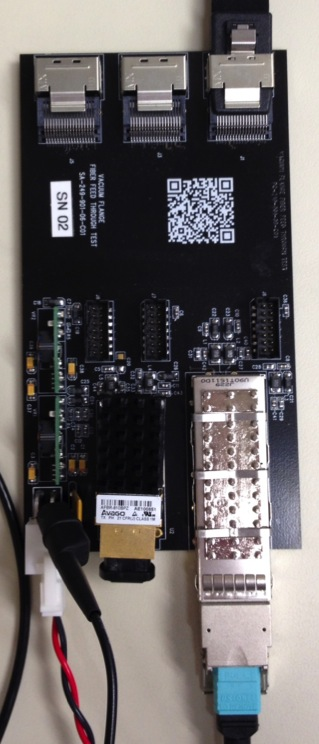
\includegraphics[angle=90,width=\textwidth]{detector/figs/flangeboard}
    \caption{One HPS signal flange board.
    The left side of the board operates in vacuum, and has three mini-SAS electrical connectors for high-speed data cables, which connect to the FEBs.
The right side of the board operates in air, and has two MPO multi-fiber connectors for data and control signals.}
    \label{fig:flangeboard}
\end{figure}

\begin{figure}[ht]
    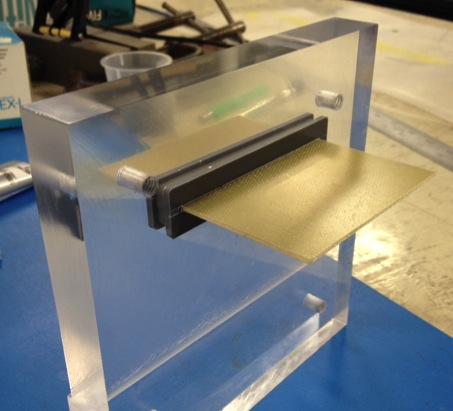
\includegraphics[width=\textwidth]{detector/figs/flangeboard_test}
    \caption{Test of the flange board potting process.}
    \label{fig:flangeboard_test}
\end{figure}

\begin{figure}[ht]
    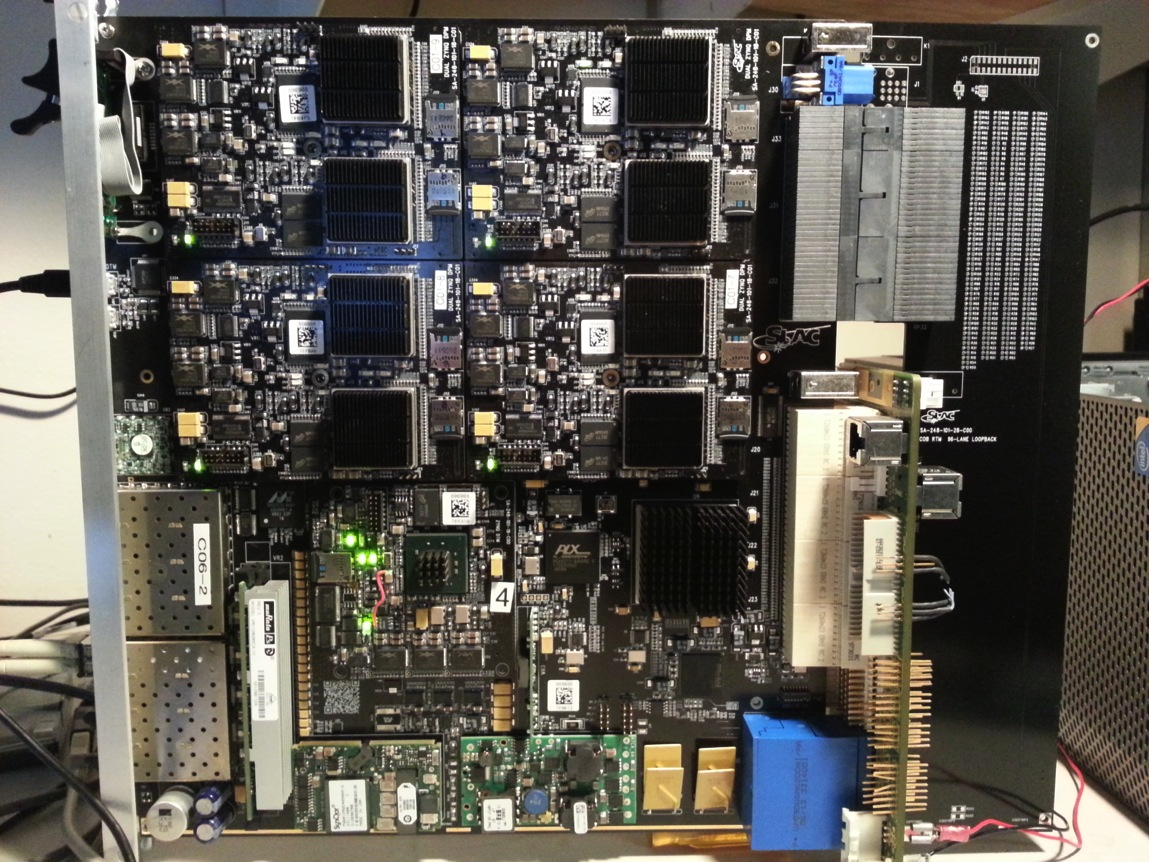
\includegraphics[width=\textwidth]{detector/figs/rce}
    \caption{The RCE system. The COB (Cluster On Board) blade on the left hosts four RCE (Reconfigurable Cluster Element) daughterboards, which perform the data processing. The RTM (Rear Transition Module) on the right interfaces with fibers carrying data from the flange boards. The COB and RTM would normally be slotted in an ATCA crate.}
    \label{fig:rce}
\end{figure}


\section{Electromagnetic Calorimeter and Trigger}
\begin{figure}[ht]
    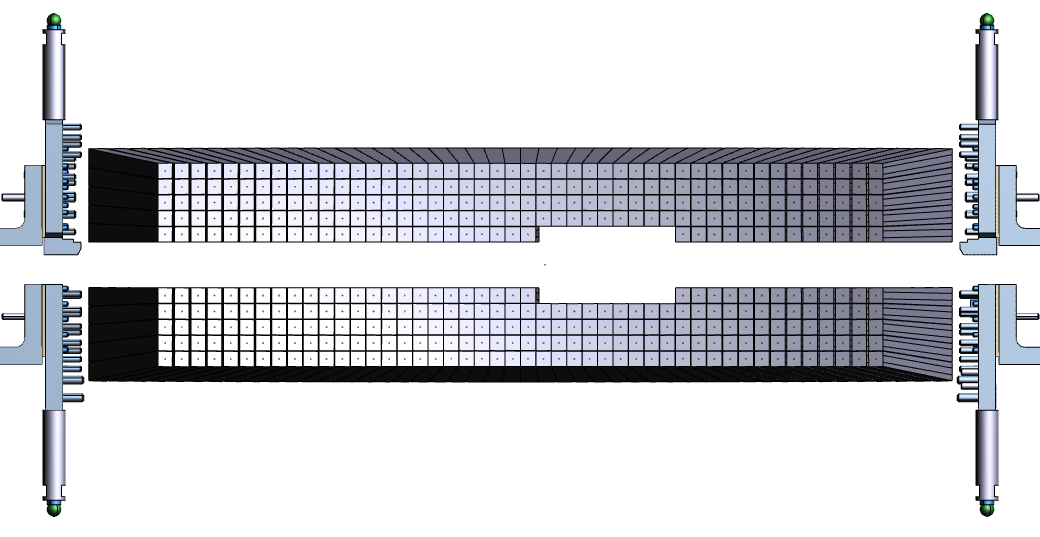
\includegraphics[width=\textwidth]{detector/figs/ECal}
    \caption{Beam's-eye-view of the ECal.}
    \label{fig:ecal}
\end{figure}

\begin{figure}[ht]
    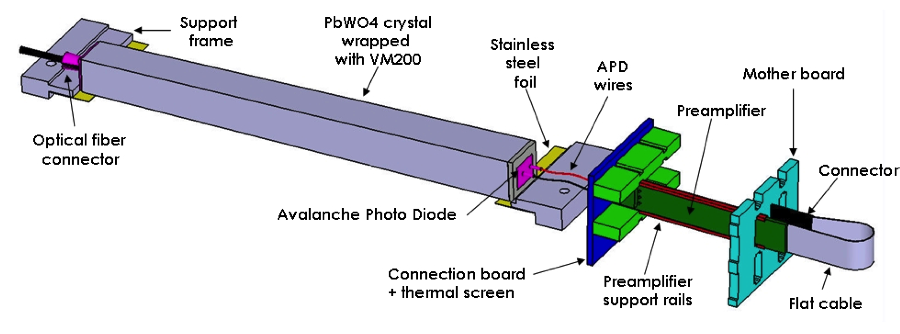
\includegraphics[width=\textwidth]{detector/figs/ecal_module}
    \caption{One ECal crystal with its readout electronics. The optical fiber was used in the CLAS IC for calibration and monitoring, but was removed for HPS. HPS uses LEDs mounted directly in front of the crystals.}
    \label{fig:ecal_module}
\end{figure}

\subsection{Trigger Cuts}
\label{sec:trigger_cuts}

\begin{table}[h]
    \begin{center}
        \begin{tabular}{lc}   
            \hline \hline
            Cluster energy & $54<E<630$ MeV \\
            Energy sum & $180<E_{top}+E_{bot}<860$ MeV \\
            Energy difference & $|E_{top}-E_{bot}|<540$ MeV \\
            Coplanarity & $|\phi_{top}-\phi_{bot}-180^\circ|<30^\circ$ \\
            Energy-distance cut & $E_{low}+(5.5\text{ MeV/mm})r_{low}>600$ MeV \\
            \hline \hline
        \end{tabular}
        \caption{Trigger cuts for the ``pairs-1'' trigger.}
        \label{tab:trigger_cuts} 
    \end{center}
\end{table}

